\section*{Appendix}\label{sec:appendix}

\subsection*{A. Reinforcement-learning configuration (Sec.~\ref{subsec:rl})}
\begin{table}[H]
    \caption{Reinforcement-learning training hyperparameters and environment settings
    (Aldo Patrone).}
    \centering
    \renewcommand{\arraystretch}{1.2}
    \tiny
    \begin{tabular}{lll}
        \toprule
        \textbf{Setting} & \textbf{REINFORCE} & \textbf{MaskablePPO} \\
        \midrule
        Policy        & per-candidate MLP & MlpPolicy \\
        Hidden layers & $24$ & $64$-$64$ \\
        Learning rate & $0.05$ & $3\cdot10^{-4}$ \\
        Discount $\gamma$ & $0.99$ & $0.99$ \\
        Entropy bonus & $0.01$ & default \\
        Training      & $500$ ep.\ $\times\,600$ & $600\mathrm{k}$ steps \\
        Rollout       & full-episode & $n=2048$, batch $256$ \\
        Seed          & $1$ & $1$ \\
        \midrule
        \multicolumn{3}{l}{\textit{Environment and reward (shared)}} \\
        Per-candidate features & \multicolumn{2}{l}{$5$} \\
        Mean interarrival      & \multicolumn{2}{l}{$1000$ s} \\
        Case length            & \multicolumn{2}{l}{$8$ to $21$ activities} \\
        Max postpone           & \multicolumn{2}{l}{$3$} \\
        Reward                 & \multicolumn{2}{l}{$1/(\mathrm{CT}/3600+1)$ + Gini shaping} \\
        Fairness weight        & \multicolumn{2}{l}{$W_{\mathrm{fair}}=5.0$} \\
        Postpone penalty       & \multicolumn{2}{l}{$-0.5$} \\
        \midrule
        \multicolumn{3}{l}{\textit{Sim-in-the-loop variant (PPO on the integrated simulator)}} \\
        Init                   & \multicolumn{2}{l}{warm-started from the REINFORCE policy} \\
        Update                 & \multicolumn{2}{l}{PPO-style: value critic, GAE $\lambda=0.95$, clip $0.2$} \\
        Iterations             & \multicolumn{2}{l}{$200$ (one simulator episode each)} \\
        Reward                 & \multicolumn{2}{l}{dense scale-invariant Gini + progress} \\
        \bottomrule
    \end{tabular}
    \label{tab:rl_hparams}
\end{table}

\begin{figure}[H]
    \centering
    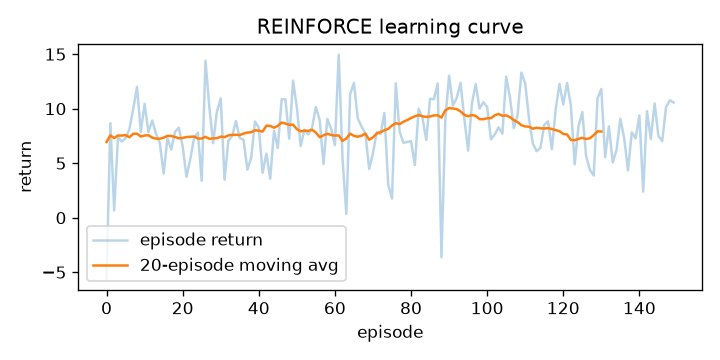
\includegraphics[width=\columnwidth]{figures/rl_learning_curve.png}
    \caption{REINFORCE learning curve (Aldo Patrone). The episode return rises as the
    per-candidate policy learns the disclosed cycle-time and fairness objective.}
    \label{fig:rl_curve}
\end{figure}
\FloatBarrier

\subsection*{B. Allocation method comparison (Sec.~\ref{ssub:rl-eval})}
\begin{figure}[H]
    \centering
    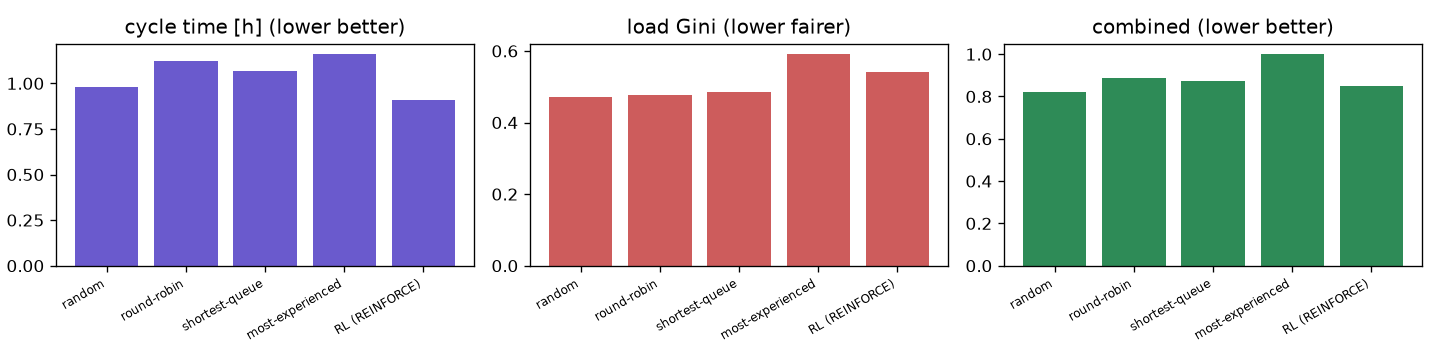
\includegraphics[width=\columnwidth]{figures/allocation_comparison.png}
    \caption{Allocation methods on the controlled case-based environment (Aldo Patrone):
    cycle time, load Gini and combined score. The robust verdict over the integrated
    simulator and multiple seeds is in Table~\ref{tab:alloc_sim}.}
    \label{fig:alloc_cmp_plot}
\end{figure}
\FloatBarrier

\subsection*{C. Resource model diagnostics (Sec.~\ref{subsec:resources})}
\begin{figure}[H]
    \centering
    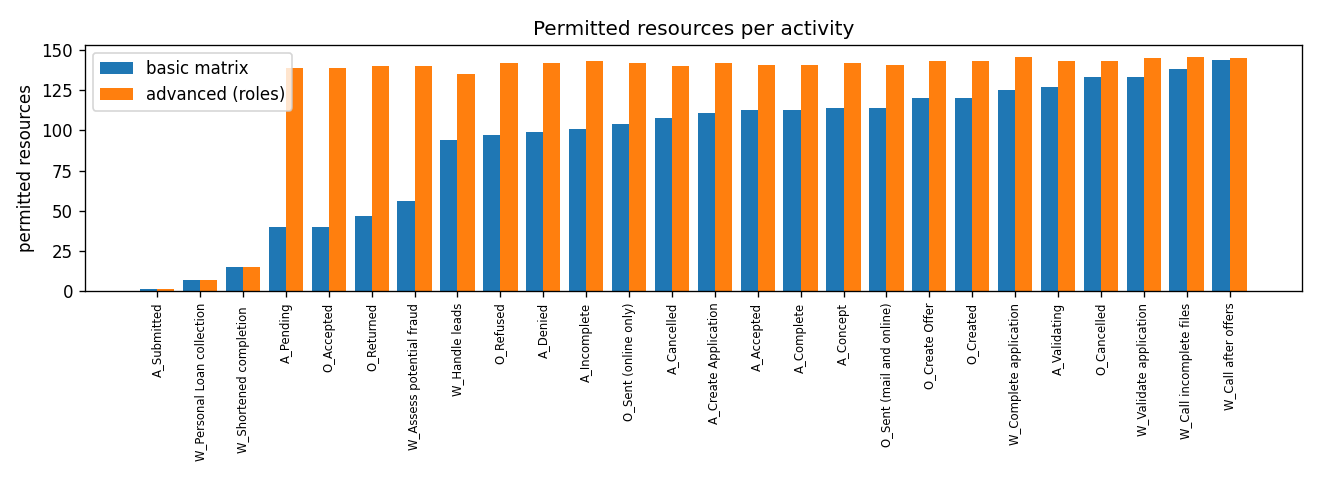
\includegraphics[width=\columnwidth]{figures/permissions_basic_vs_advanced.png}
    \caption{Permitted resources per activity (Aldo Patrone), basic resource-activity
    matrix versus advanced role-based model. Role discovery generalizes permissions
    while the observed-performer floor keeps every activity covered.}
    \label{fig:perm_breadth}
\end{figure}

\begin{figure}[H]
    \centering
    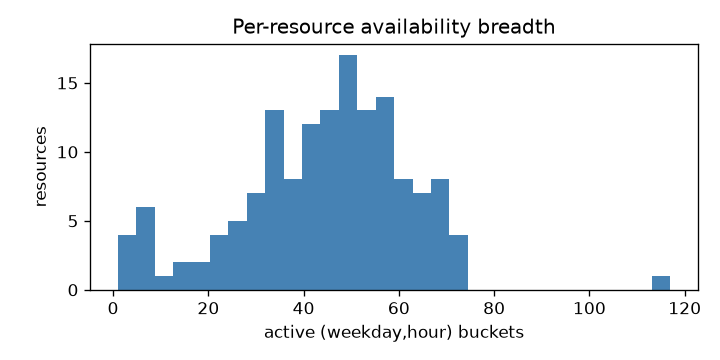
\includegraphics[width=\columnwidth]{figures/availability_calendar_sizes.png}
    \caption{Per-resource availability breadth (Aldo Patrone), the number of active
    (weekday, hour) buckets in each learned calendar out of $168$.}
    \label{fig:cal_sizes}
\end{figure}

\begin{figure}[H]
    \centering
    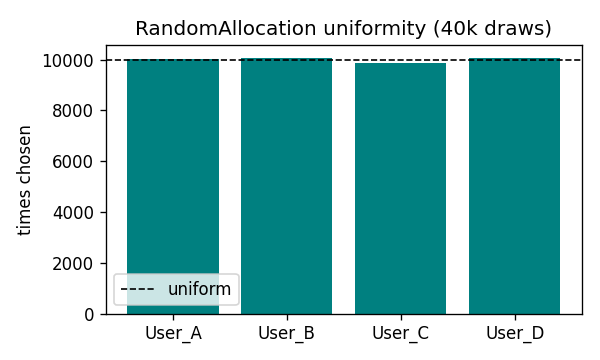
\includegraphics[width=\columnwidth]{figures/allocation_uniformity.png}
    \caption{RandomAllocation uniformity (Aldo Patrone) over a four-resource candidate
    set across $40000$ draws, confirming the unbiased Part~I baseline.}
    \label{fig:alloc_unif}
\end{figure}
\FloatBarrier
